\documentclass[tikz,border=10pt]{standalone}
\usetikzlibrary{arrows.meta, positioning}

\begin{document}
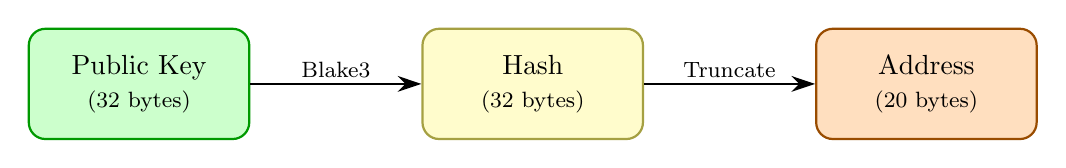
\begin{tikzpicture}[
  every node/.style={align=center},
  % Nodes (data boxes) - rounded, colored fills
  node/.style={rectangle, draw=black, thick, rounded corners=6pt, minimum width=2.8cm, minimum height=1.4cm, font=\normalsize},
  % Edges (operations) - smaller, distinct style on arrows
  edge/.style={-{Stealth[length=3mm, width=2mm]}, thick, draw=black},
  edgelabel/.style={font=\footnotesize, fill=white, inner sep=2pt}
]

% === NODES (Data) ===

% Public Key
\node[node, fill=green!20, draw=green!60!black] (pubkey) at (0, 0) {Public Key\\{\footnotesize (32 bytes)}};

% Hash Output
\node[node, fill=yellow!20, draw=yellow!60!black] (hash) at (5, 0) {Hash\\{\footnotesize (32 bytes)}};

% Address
\node[node, fill=orange!25, draw=orange!60!black] (address) at (10, 0) {Address\\{\footnotesize (20 bytes)}};

% === EDGES (Operations) ===

% Edge: Public Key -> Hash (Blake3)
\draw[edge] (pubkey.east) -- node[edgelabel, above] {Blake3} (hash.west);

% Edge: Hash -> Address (Truncate)
\draw[edge] (hash.east) -- node[edgelabel, above] {Truncate} (address.west);

\end{tikzpicture}
\end{document}
